\documentclass[conference]{IEEEtran}
\usepackage{blindtext, graphicx}

\usepackage[slovak]{babel}
\usepackage[utf8]{inputenc}
\usepackage{cite}

\usepackage{url}
\usepackage{amsmath}

\usepackage{algorithm}
\usepackage{algpseudocode}

\algnewcommand\algorithmicforeach{\textbf{for each}}
\algdef{S}[FOR]{ForEach}[1]{\algorithmicforeach\ #1\ \algorithmicdo}

% correct bad hyphenation here
\hyphenation{op-tical net-works semi-conduc-tor}

\begin{document}
%
% paper title
% can use linebreaks \\ within to get better formatting as desired
\title{Implementácia modifikovaného algoritmu SHA-1 v jazyku C (CPU) a CUDA (GPU)}

% author names and affiliations
% use a multiple column layout for up to three different
% affiliations
\author{\IEEEauthorblockN{Peter Kaňuch}
\IEEEauthorblockA{Fakulta informatiky a informačných technológií\\
Slovenská Technická Univerzita\\
Slovenská republika, 841 04 Bratislava IV\\
Email: xkanuch@stuba.sk}}

% use for special paper notices
%\IEEEspecialpapernotice{(Invited Paper)}

% make the title area
\maketitle

\begin{abstract}
%\boldmath
V posledných rokoch sa grafické procesory začali dostávať do popredia nie len na spracovanie obrazu, ale aj na vykonávanie, či spracovanie rôznych náročných výpočtových úloch. Keďže GPU architektúra bola navrhnutá a optimalizovaná pre paralelné spracovanie inštrukcií a dát, zatiaľ čo CPU sú optimalizované pre rýchle sequenčné spracovanie toku programu. V tomto článku porovnáme základnú architektúru CPU a GPU. Vysvetlíme princíp fungovania algoritmu SHA-1 a jeho modifikovanej paralelizovanej verzii. Daný algoritmus implementujeme v programovacom jazyku C pre klasické a v jazyku CUDA pre grafické procesory. Výsledky ukazujú porovnanie nameraných časov vykonávania daného algoritmu na CPU a GPU. V závere diskutujeme, prečo ešte v súčasnosti neexistuje automatický paralelizmus a automatické vykonávanie výpočtovo náročných úloch na grafických procesoroch.
\end{abstract}

\begin{IEEEkeywords}
SHA-1, Modified SHA-1, CPU architecture, GPU architecture, Automatic parallelism for GPU 
\end{IEEEkeywords}

\IEEEpeerreviewmaketitle

\section{Úvod}


\section{CPU verzus GPU architektúra}

Aj keď sa zdá, že grafické procesory by mohli svojou výkonnosťou nahradiť klasické počítačové procesory, nie je tomu tak. CPU boli navrhnuté pre dosiahnutie čo najlepšieho výkonu pre sequenčné spracovanie dát, grafické procesory boli navrhnuté za účelom paralelného vykonávania inštrukcií. Pri porovnaní týchto procesorov CPU majú/sú \cite{gpuRowe}:

\begin{enumerate}
	\item{menej výpočtových jednotiek}
	\item{optimalizované pre sériové operácie}
	\item{nízku toleranciu latencie}
	\item{podporu pre paralelné spracovanie (novšie verzie)}
\end{enumerate}

a GPU:

\begin{enumerate}
	\item{viac výpočtových jednotiek}
	\item{vstavané pre paralelné operácie}
	\item{vysokú toleranciu latencie}
	\item{vysokú priepustnosť}
	\item{lepšiu logiku riadenia}
\end{enumerate}


\begin{figure}[!h]
\centering
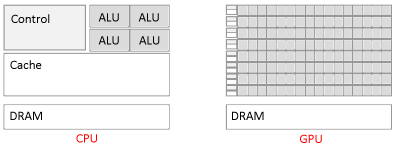
\includegraphics[width=2.5in]{img/CPU-GPU-3}
\caption{CPU vz. GPU}
\end{figure}


\subsection{Architektúra počítačových procesorov}

CPU (Central Processing Unit) alebo aj procesor, je hlavný komponent počítača, ktorý načítava, spracováva a vykonáva inštrukcie nad rôznymi dátami. Procesor pozostáva z dvoch hlavných častí:

\begin{itemize}
	\item{kontrolná jednotka (CU)}
	\item{aritmeticko-logická jednotka (ALU)}
\end{itemize}

Základný procesor pozostáva z piatich fáz \cite{hennessy2007compute}: 

\begin{itemize}
	\item{IF (Instruction Fetch) - fáza, v ktorej sa načítava inštrukcia z pamäte do procesora na základe adresy v registry IP/PC (instruction pointer/program counter) a jeho následnej inkrementácii na ďalšiu adresu }
	\item{ID (Instruction Decode) - zabezpečuje dekódovanie inštrukcie}
	\item{EX (Execute) - fáza, v ktorej procesor vykonáva rôzne výpočty pomocou ALU}
	\item{MEM (Memory Access) - v tejto fáze, procesor pristupuje do pamäte pre načítanie alebo uloženie dát}
	\item{WB (Write Back) - procesor zapíše výsledky(hodnoty z predošlých fáz vypočítané v ALU) alebo hodnoty načítané z pamäte v predchádzajúcej fáze do registrov}
\end{itemize}

\begin{figure}[!h]
\centering
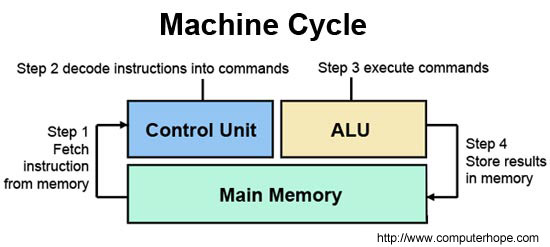
\includegraphics[width=3.5in]{img/CPU-cycle}
\caption{Základný cyklus procesora}
\end{figure}

Takáto základná architektúra bola postupne vylepšovaná rôznymi mechanizmami (prúdovým spracovaním, detekciou a riešením hazardov, či závislostí, predikciou vetvenia a iné) pre dosiahnutie čo najlepšieho výkonu, t.j. dosiahnutie čo najmenšieho CPI (CPI - počet cyklov na inštrukciu).

Jedným z vylepšení procesora je \textit{prúdové spracovanie.} To spočíva v tom, že v každom hodinovom cykle procesora dokážeme začať spracovávať novú inštrukciu \cite{hennessy2007compute}. Tým dokážeme znížiť vykonávanie jednej inštrukcie z piatich cyklov  na hodnotu blízkej jedna. Nie je to však jednoduché. Vznikajú takzvané \textit{hazardy} a \textit{závislosti v programe}. 

Ďalším vylepšením procesora, kedy inžinieri chceli zvýšiť výkonnosť procesora, bolo vymyslením \textit{Hyper-threading}-u. Hyper-threading vytvára z jedného fyzického, viacero logických procesorov \cite{hyperthreading}. Procesor podporujúci danú technológiu si dokáže zapamätať viacero stavov procesora pomocou pridanej kompletnej sady jednotlivých registrov (základných, kontrolných, ...).  
Princíp fungovania je jednoduchý: V každom čase sa spracováva len jedna úloha. Procesor však dokáže veľmi rýchlo prepínať medzi jednotlivými úlohami, čo vytvára pocit, že bežia súčasne. \newline
Základnou nevýhodou hyper-threading-u je, že ostatné súčasti procesora (ALU, MMU, FPU, SIMD) zdieľa medzi úlohami (viď obr. \ref{img} \cite{picture}) \cite{hyper2}. Preto tento spôsob zlepšenia nám nezvýši výkon pri výpočtovo náročných úlohách (napr. násobenie matíc).

\begin{figure}[!h]
\centering
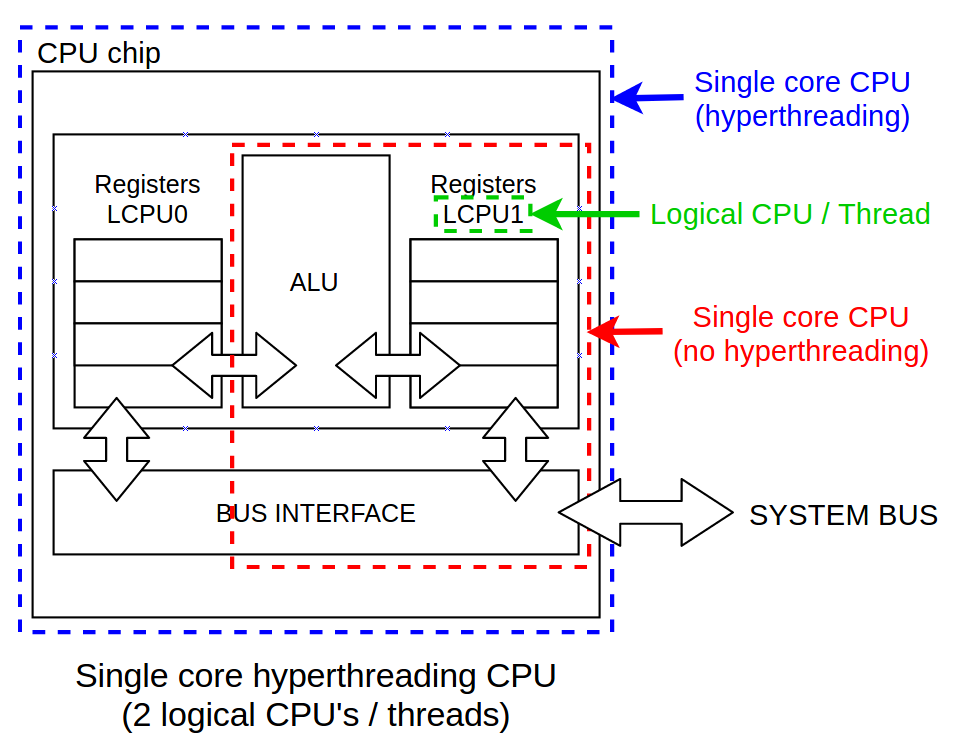
\includegraphics[width=2.75in]{img/hyper}
\caption{1-jadrový procesor s hyper-threading \label{img}}
\end{figure}

Iným vylepšením procesora je pridanie viacerých jadier procesora na jeden spoločný čip (viď obr. \ref{quad}\cite{picture}). Týmto spôsobom sa nám znásobi aj počet vykonávacich jednotiek 
čím dosiahneme aj znásobenie výpočtového výkonu. Súčasné bežné procesory v prenosných počítačoch obsahujú dve až štyri jadrá. Najvýkonnejšie procesory pozostávajú zo šiestich a viac jadier (12 až 18).  

\begin{figure}[!h]
\centering
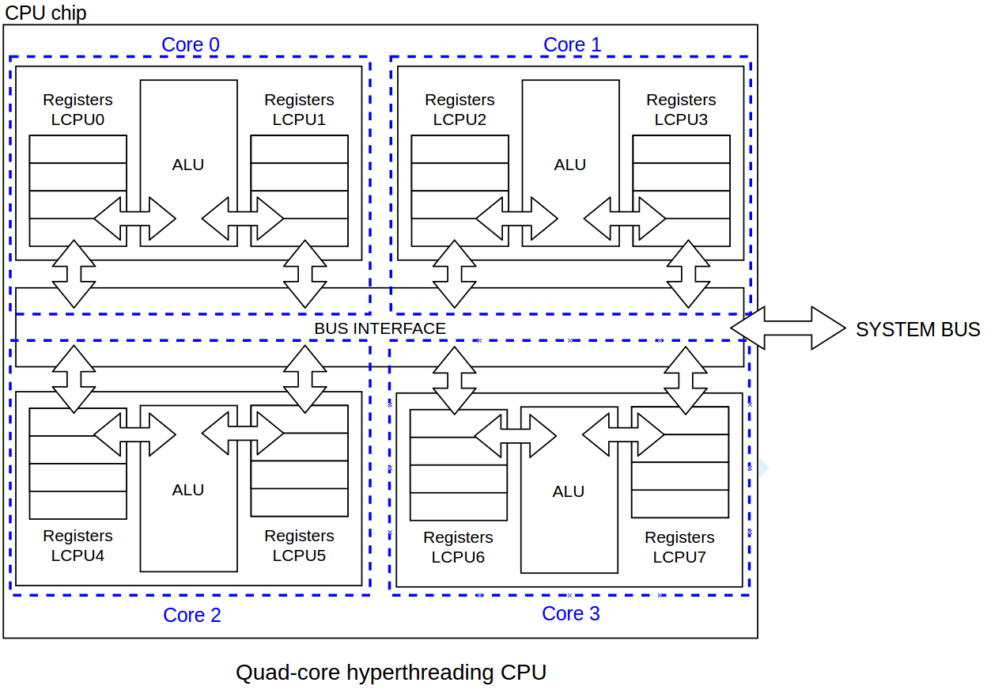
\includegraphics[width=3in]{img/quad}
\caption{4-jadrový procesor s hyper-threading \label{quad}}
\end{figure}

\subsection{Architektúra grafických procesorov}

Grafické procesory sú navrhnuté tak, aby čo najrýchlesjšie dokázali vykonať paralelizovateľný kód. Napríklad vykonať rovnaké inštrukcie nad rôznymi dátami. Do návrhu boli zahrnuté 3 myšlienky \cite{GPU2011Fatahalian}: 

\begin{enumerate}
	\item{Pre GPU odstrániť tie časti CPU, ktoré umožňujú rýchle sequenčné výkonávanie inštrukcií.}\\
	\item{Znížiť náročnosť riadenia inštrukcií vo viacerých ALU.}\\
	\item{Predchádzať hazardom pomocou začatia vykonávania iného bloku.}
\end{enumerate}

\begin{figure}[!h]
\centering
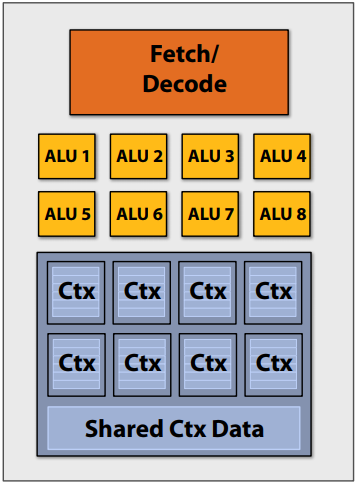
\includegraphics[width=2.1in]{img/GPU-core}
\caption{Jedno jadro grafického procesora \label{core}}
\end{figure}

Grafický procesor pozostáva z nasledujúcich častí \cite{tatourian}:

\begin{enumerate}
	\item{Globálna pamäť}
	\item{Multi-procesor - ten sa skladá z:}
	\begin{itemize}
		\item{Kontrolné jednotky}
		\item{Registre}
		\item{Výkonné jednotky}
		\item{Cache pamäte}
	\end{itemize}
\end{enumerate}

Programy, napísané pre grafické procesory, nevedia pristupovať k dátam uloženým v hlavnej pamäti \cite{gpuRowe}. Taktiež, GPU boli navrhnuté pre rýchle paralelné spracovanie dát a nepodporujú niektoré funkcie operačného systému. Z tohto dôvodu musia CPU a GPU procesory spolupracovať. Za vykonanie programu na grafike je zodpovedný CPU \cite{tatourian}. Ten má za úlohu:

\begin{itemize}
	\item{Prekopírovať dáta potrebné pre vykonanie programu z hlavnej pamäte do video pamäte.}
	\item{Vložiť program (GPU kernel) naprogramovaný programátorom na grafický procesor.}
	\item{Po dokončení a spracovaní dát nakopírovať späť výsledné dáta z video pamäte do hlavnej pamäte}
\end{itemize}

\begin{figure}[!h]
\centering
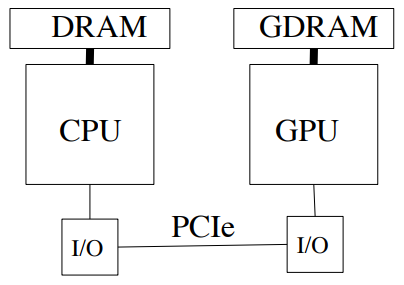
\includegraphics[width=1.5in]{img/CPU+GPU}
\caption{Spojenie CPU a GPU}
\end{figure}

%**********************************************************************************************************************
\section{Opis riešenia}

Pre porovnanie časov vykonávania programu na CPU a GPU, sme sa rozhodli naprogramovať algoritmus SHA-1 v jazyku C pre CPU a v jazyku CUDA pre grafické procesory. Klasický algoritmus SHA však nie je paralelizovateľný, a preto sme implementovali jednu z jeho modifikácií pre paralelné spracovanie. Výber problému nie je veľmi vhodný vzhľadom na porovnanie architektúry procesorov, keďže daný problém nepozostáva zo zložitých aritmeticko-logických operácií.

\subsection{Algoritmus SHA-1 a jeho modifikácia}

Všeobecný algoritmus SHA pozostáva z nasledujúcich krokov:

\begin{enumerate}
	\item{Predspracovanie}
	\begin{itemize}
		\item{Zarovnanie správy}
		\item{Rozdelenie na bloky}
		\item{Nastavenie počiatočného výsledku hash-u}\\
	\end{itemize}
	\item{Výpočet hash-u}
\end{enumerate}

Princíp fungovania SHA: 
\begin{enumerate}
	\item{Zarovnanie správy pomocou nulových bajtov a doplnením veľkosti správy na koniec}
	\item{Rozdelenie správy na bloky o veľkosti 64 bajtov}
	\item{Nastavenie počiatočného výsledku hash-u}
	\item{Vykonanie operácií a pripojenie medzivýsledku ku finálnemu hashu pre každý blok}
\end{enumerate}

\begin{algorithm}
   \caption{SHA-1 \cite{sha-algo}}
    \begin{algorithmic}[1]
      \Function{SHA}{$Message$ $M$}

        \State padding(M) \Comment{Put zero bytes into message and its size at the end}
        \State  Set ${H_0}$ \Comment{Initial value of hash}
     	\ForEach {$block \in \mathcal M $} \Comment{512 bit block size}
     		\For{$i = 0$ to $15$}
     			\State $W_i = M_i$
     		\EndFor
     		\For{$i = 16$ to $79$}
     			\State $W_i = ROTL^1(W_{i-3} \oplus W_{i-8} \oplus W_{i-14} \oplus W_{i-16})$
     		\EndFor
		\State Set ${a, b \ldots e}$ with ${H_{0..4}^{i-1}}$
		\For{$i = 0$ to $79$} \Comment{f = Ch for i == 0 ... 19; Parity for i == 20 ... 39 \& 60 ... 79; Maj for i == 40...59}
			\State  $T = ROTL^5(a) + f(b,c,d) + e + K_i + W_i)$
			\State  $e = d$
			\State  $d = c$
			\State  $c = ROTL^{30}(b)$
			\State  $b = a$
			\State  $a = T$
     		\EndFor		
     	\EndFor
   	\State ${H_{0..4}^{i-1}}$ = ${a, b \ldots e}$ + ${H_{0..4}^{i-1}}$
       \EndFunction
\end{algorithmic}
\end{algorithm}


\begin{figure}[!h]
\centering
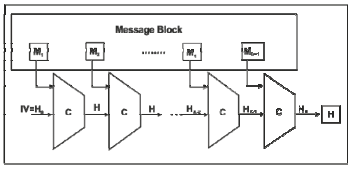
\includegraphics[width=3in]{img/SHA}
\caption{Grafické znázornenie klasického algoritmu SHA}
\end{figure}

Princíp fungovania modifikovanej SHA: 
\begin{enumerate}
	\item{Zarovnanie správy pomocou nulových bajtov a doplnením veľkosti správy na koniec}
	\item{Rozdelenie správy na bloky o veľkosti 64 bajtov}
	\item{Pre každý blok}
	\begin{enumerate}
		\item{Nastavenie počiatočnej hodnoty}
		\item{Vykonanie operácií}
		\item{Pripojenie výsledku k počiatočnej hodnote}
	\end{enumerate}
	\item{Spojenie výsledkov jednotlivých blokov}
	\item{Ak veľkosť bloku nerovná sa 20 bajtov $\implies$ pokračuj v bode 1.}
\end{enumerate}

\begin{figure}[!h]
\centering
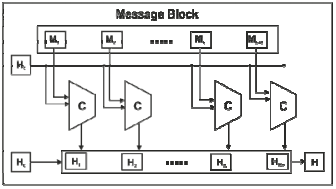
\includegraphics[width=3in]{img/MSHA}
\caption{Grafické znázornenie modifikovaného algoritmu SHA}
\end{figure}


\subsection{Vlastnosti SHA-1 a jeho modifikovanej verzie}

Pre všetky hashovacie funkcie je dôležité spĺňať nasledujúce vlastnosti \cite{CHF}:

\begin{itemize}
	\item{Ireverzibilnosť hashu (Preimage resistance) - pre daný hash je ťažké nájsť správu, po ktorej zahashovaní dostaneme pôvodný hash}
	\item{Odolnosť voči kolíziám - je ťažké nájsť také dve rôzne správy, ktorých výsledky hashu sa rovnajú}
\end{itemize}

Daný modifikovaný algoritmus SHA-1 by mal spĺňať všetky vlastnosti hashovacích funkcií, viď článok\cite{MSHA}.


\subsection{Testovacie prostredie a implementácia}

\section{Výsledky a grafické porovnanie}

\section{Záver}


\appendices
\section{aaa}



% use section* for acknowledgement
\section*{Acknowledgment}


The authors would like to thank...


% Can use something like this to put references on a page
% by themselves when using endfloat and the captionsoff option.
\ifCLASSOPTIONcaptionsoff
  \newpage
\fi




\begin{thebibliography}{1}

\bibitem{hennessy2007compute}
HENNESSY, John L.; PATTERSON, David A. Computer architecture: a quantitative approach. Elsevier, 2007.

\bibitem{tatourian}
TATOURIAN, Alan. Nvidia gpu architecture and cuda programming environment. URL http://code. msdn. microsoft. com/windowsapps/NVIDIA-GPU-Architecture-45c11e6d, 2013.

\bibitem{hyperthreading}
PRECOMPUTATION, Speculative. Hyper-Threading Technology.

\bibitem{hyper2}Intel Pentium 4 3.06 GHz with Hyper-Threading support, \url{http://ixbtlabs.com/articles2/pentium43ghzht/}, 12.11.2017.

\bibitem{GPU2011Fatahalian}How a GPU Works - Kayvon Fatahalian 15-462 (Fall 2011), \url{https://www.cs.cmu.edu/afs/cs/academic/class/15462-f11/www/lec_slides/lec19.pdf}, 12.11.2017.

\bibitem{picture}Differences between physical CPU vs logical CPU vs Core vs Thread vs Socket, \url{http://www.daniloaz.com/en/differences-between-physical-} \url{cpu-vs-logical-cpu-vs-core-vs-thread-vs-socket/}, 12.11.2017.

\bibitem{gpuRowe}The Continuing Importance of GPUs For More Than Just Pretty Pictures - Jeff Rowe, \url{https://www10.mcadcafe.com/blogs/jeffrowe/2017/03/16/the-continuing-importance-of-gpus-for-more-than-just-pretty-pictures/}, 12.11.2017

\bibitem{sha-algo}GALLAGHER, Patrick; DIRECTOR, Acting. Secure hash standard (shs). FIPS PUB, 1995, 180-3.

\bibitem{CHF}ROGAWAY, Phillip; SHRIMPTON, Thomas. Cryptographic hash-function basics: Definitions, implications, and separations for preimage resistance, second-preimage resistance, and collision resistance. In: International Workshop on Fast Software Encryption. Springer, Berlin, Heidelberg, 2004. p. 371-388.

\bibitem{MSHA}KISHORE, Neha; KAPOOR, Bhanu. An efficient parallel algorithm for hash computation in security and forensics applications. In: Advance Computing Conference (IACC), 2014 IEEE International. IEEE, 2014. p. 873-877.

\end{thebibliography}






\end{document}


